To illustrate the problem of cross-domain optimization, we examine two streaming dataflows that share common parts and can be optimized simultaneously. Our example is based on the NEXMark~\cite{tucker2008nexmark} benchmark, which models an online auction platform where users can start auctions for items and bid on them.

The first dataflow is analytical. It calculates the number of participants for each auction and can be defined by an SQL query:
\begin{lstlisting}[language=SQL]
SELECT auction.id, COUNT(person) FROM bid
INNER JOIN person ON bidder = person.id
INNER JOIN auction ON auction = auction.id
GROUP BY auction.id
\end{lstlisting}

The second dataflow is fraud detection. Online auctions often face the fraud problem and need to monitor corresponding metrics, e.g., the ratio of correlated bids. Within our model, the metric can be computed using only bids data.
However, metric values can be more precise if we use information about personal ratings or item popularity.

Therefore, we have a shared execution graph shown in Figure~\ref{running_example}. Note that painted nodes can be permuted depending on the runtime statistics to achieve better performance. Joins can be permuted based on the rates of the input streams. Computation of the fraud detection metric can be placed after joins for better precision if the latency satisfies the business requirements.

TODO(rewrite)

\begin{figure}[h!]
    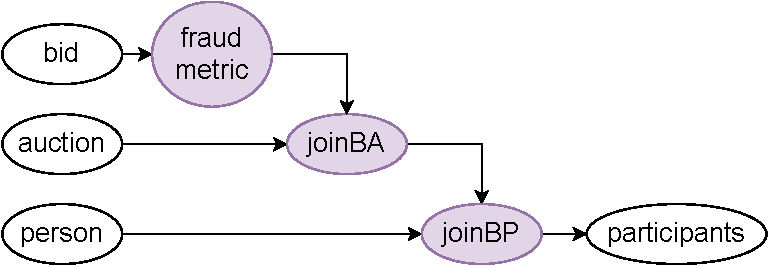
\includegraphics[width=0.4\textwidth]{images/poster.pdf}
    \caption{A possible execution graph for running example.}
    \label{running_example}
\end{figure}
